 \documentclass{beamer}
%
% Choose how your presentation looks.
% For more themes, color themes and font themes, see:
% http://deic.uab.es/~iblanes/beamer_gallery/index_by_theme.html
%
\mode<presentation>
{
  \usetheme{Madrid}      % or try Darmstadt, Madrid, Warsaw, ...
  \usecolortheme{seahorse} % or try albatross, beaver, crane, ...
  \usefonttheme{serif}  % or try serif, structurebold, ...
  \setbeamertemplate{navigation symbols}{}
  \setbeamertemplate{caption}[numbered]
  \usepackage{amsmath}
  \usepackage{tcolorbox}
  \usepackage[export]{adjustbox}
  \tcbuselibrary{most}
  \usepackage{arydshln}
  \usepackage{tikz}
  \usetikzlibrary{plotmarks}
  \usepackage{pgfplots}
  \newcommand{\Ivec}[1]{\mbox{\boldmath $#1$}}
    \usepackage[normalem]{ulem}
    % \usepackage{tipa}
    \newcommand{\git}{\texttt{\textbf{git}}\xspace}
    \usepackage{listings}
} 


\definecolor{myblue}{RGB}{65,105,225} 
\definecolor{myorange}{RGB}{250,190,0}

\setbeamercolor{structure}{fg=white,bg=myorange}
\setbeamercolor*{palette primary}{fg=myblue,bg=myorange}
\setbeamercolor*{palette secondary}{fg=white,bg=myblue}
\setbeamercolor*{palette tertiary}{bg=myblue,fg=white}
\setbeamercolor*{palette quaternary}{fg=white,bg=myorange!50}

\setbeamercolor{frametitle}{fg=black!90!myblue}

\setbeamercolor{section in head/foot}{fg=white,bg=myblue}
\setbeamercolor{author in head/foot}{fg=black,bg=myorange}
\setbeamercolor{title in head/foot}{fg=white,bg=myblue}

\setbeamertemplate{navigation symbols}{}

\setbeamertemplate{itemize/enumerate body begin}{\large}
\setbeamertemplate{itemize/enumerate subbody begin}{\large}


\defbeamertemplate*{headline}{mytheme}
{%
  \begin{beamercolorbox}[ht=2.25ex,dp=3.75ex]{section in head/foot}
    \insertnavigation{\paperwidth}
  \end{beamercolorbox}%
}%

\defbeamertemplate*{footline}{mytheme}
{
  \leavevmode%
  \hbox{%
  \begin{beamercolorbox}[wd=.5\paperwidth,ht=2.25ex,dp=1ex,right]{author in head/foot}%
    \usebeamerfont{author in head/foot}\insertshortauthor\hspace*{2em}
  \end{beamercolorbox}%
  \begin{beamercolorbox}[wd=.5\paperwidth,ht=2.25ex,dp=1ex,left]{title in head/foot}%
    \usebeamerfont{title in head/foot}\hspace*{2em}\insertshortsubtitle\hspace*{2em}
    \insertframenumber{} / \inserttotalframenumber
  \end{beamercolorbox}}%
  \vskip0pt%
}

\usepackage[english]{babel}
\usepackage[utf8x]{inputenc}
\usepackage{xcolor}
\usepackage{listings}
\usepackage{pgf}  
\usepackage{textpos}
\usepackage{tabulary}
\usepackage{scrextend}
\usepackage{hyperref}
\usepackage{setspace}
\usepackage{rotating}
\lstset
{
    language=[LaTeX]TeX,
    breaklines=true,
    basicstyle=\tt\scriptsize,
    %commentstyle=\color{green}
    keywordstyle=\color{blue},
    %stringstyle=\color{black}
    identifierstyle=\color{magenta},
}
\newcommand{\bftt}[1]{\textbf{\texttt{#1}}}
%\newcommand{\comment}[1]{{\color[HTML]{008080}\textit{\textbf{\texttt{#1}}}}}
\newcommand{\cmd}[1]{{\color[HTML]{008000}\bftt{#1}}}
\newcommand{\bs}{\char`\\}
\newcommand{\cmdbs}[1]{\cmd{\bs#1}}
\newcommand{\lcb}{\char '173}
\newcommand{\rcb}{\char '175}
\newcommand{\cmdbegin}[1]{\cmdbs{begin\lcb}\bftt{#1}\cmd{\rcb}}
\newcommand{\cmdend}[1]{\cmdbs{end\lcb}\bftt{#1}\cmd{\rcb}}

\newcommand{\wllogo}{\textbf{Overleaf}}

\usepackage{hyperref}
\hypersetup{
    colorlinks=true,
    linkcolor=blue,
    filecolor=magenta,      
    urlcolor=cyan,
    pdftitle={Overleaf Example},
    pdfpagemode=FullScreen,
    }

\urlstyle{same}

% this is where the example source files are loaded from
% do not include a trailing slash
\newcommand{\fileuri}{https://raw.githubusercontent.com/GiancarloSucci/UniBo.IDSEPC.A2022/main/A2022.IDSEPCLaTeX/}

\newcommand{\perche}{perch\'{e}}
\newcommand{\affinche}{affinch\'{e}}
\newcommand{\se}{s\'{e}}
\newcommand{\a}{\`{a}}
\newcommand{\est}{\`{e}}

\usepackage{stackengine}
\def\Ruble{\stackengine{.67ex}{%
  \stackengine{.48ex}{\textsf{P}}{\rule{.8ex}{.12ex}\kern.6ex}{O}{r}{F}{F}{L}%
  }{\rule{.8ex}{.12ex}\kern.6ex}{O}{r}{F}{F}{L}\kern-.1ex}



%----------------------------------------------------------------------------------------
%	TITLE PAGE
%----------------------------------------------------------------------------------------
\title[L02]{Introduzione alla data science e al pensiero computazionale\\
Lezione 6: Il modello GQM, Misurazione e Deduzione} % The short title appears at the bottom of every slide, the full title is only on the title page

\author[{\tiny Giancarlo Succi }]{Giancarlo Succi\\\\ Dipartimento di Informatica -- Scienza e Ingegneria\\Universit\`{a} di Bologna\\
\bftt{g.succi@unibo.it}
} % Your name
\institute[unibo] % Your institution as it will appear on the bottom of every slide, may be shorthand to save space

\date{} % Date, can be changed to a custom date

\setbeamertemplate{navigation symbols}{}
\AtBeginSection[]
{
        \begin{frame}<beamer>{Outline}
                \tableofcontents[currentsection]
        \end{frame}
}

\begin{document}
\begin{frame}
\titlepage % Print the title page as the first slide

\end{frame}

%=============================================

\addtobeamertemplate{frametitle}{}{%
\begin{textblock*}{10mm}(-0.01mm,-0.95cm)

\includegraphics[width=0.9cm]{unibo-logo.png}
\end{textblock*}}

%=============================================

\begin{frame}
{\centerline{Indice}}
\begin{itemize}
    \item Il concetto di misura
    \item Definizione di misure con il GQM
    \item Definizione delle ipotesi nelle sperimentazioni
    \item Verifiche empiriche
\end{itemize} 
\end{frame}


%---------------------------------------------
\begin{frame}{\centerline{}}

\begin{center}
{\Large
Introduction to Measurement \\
}
\end{center}
\end{frame}
%=============================================



%---------------------------------------------
\begin{frame}{\centerline{Definition}}


\textbf{Measurement} is the process by which numbers or symbols are assigned to attributes of entities in the real world in such a way as to describe them according to clearly defined rules
\begin{flushright}
N. Fenton and S. L. Pfleeger, 1997
\end{flushright}

\end{frame}
%=============================================

%---------------------------------------------
\begin{frame}{\centerline{Entities and Attributes}}


\begin{table}[H]
\begin{tabulary}{\textwidth}{m{5.5cm} m{5.5cm}}
\begin{itemize}    
    \item Human being
    \item Apple
    \item Computer
    \item Computer
    \item Human being
    \item ...
\end{itemize} &
\begin{itemize}    
    \item Name
    \item Weight
    \item Memory
    \item Hard Disk space
    \item Weight
    \item ...
\end{itemize}
\end{tabulary}
\end{table}
\end{frame}
%=============================================

%---------------------------------------------
\begin{frame}{\centerline{Rules}}

\begin{itemize}    
    \item The LOC measure is obtained by counting all the lines that contain at least one character, and that do not contain comments.
    \item Interpretation: C Code?
    \item Visual BASIC 4 Code?
\end{itemize}
\end{frame}
%=============================================

%---------------------------------------------
\begin{frame}{\centerline{Why Measuring?}}


\begin{itemize}
\item Lack of measurable targets (Gilb's principle)
\item Identification failure
\item Lack of quality assurance
\item Lack of consistent tool evaluation
\end{itemize}

\end{frame}
%=============================================

%---------------------------------------------
\begin{frame}{\centerline{The Measurement Advantage}}
0
\begin{table}[H]

\begin{tabulary}{\textwidth}{m{5.5cm} m{5.5cm}}
Management &
Engineering \\

\begin{itemize}    
    \item Cost
    \item Productivity
    \item Quality
    \item User satisfaction
    \item Optimisation
\end{itemize} &
\begin{itemize}    
    \item Requirements testing
    \item Fault detection
    \item Meeting goals
    \item Forecasting
\end{itemize}
\end{tabulary}
\end{table}

\end{frame}
%=============================================

%---------------------------------------------
\begin{frame}{\centerline{Scope of Measurement (partial list)}}
1
\begin{itemize}
    \item Cost and effort estimation
    \item Productivity measures and models
    \item Data collection
    \item Quality models and measures
    \item Reliability models
    \item Performance evaluation and models
    \item Structural and complexity metrics
    \item Capability-maturity assessment
    \item Management by metrics
    \item Evaluation of methods and tools
\end{itemize}
\end{frame}
%=============================================

%---------------------------------------------
\begin{frame}{\centerline{}}
2

\begin{center}
{\Large
Theory of Measurement
}
\end{center}

\end{frame}
%=============================================



%---------------------------------------------
\begin{frame}{\centerline{The Representational Theory of Measurement}}
3
Set of rules to define measurement

\begin{center}
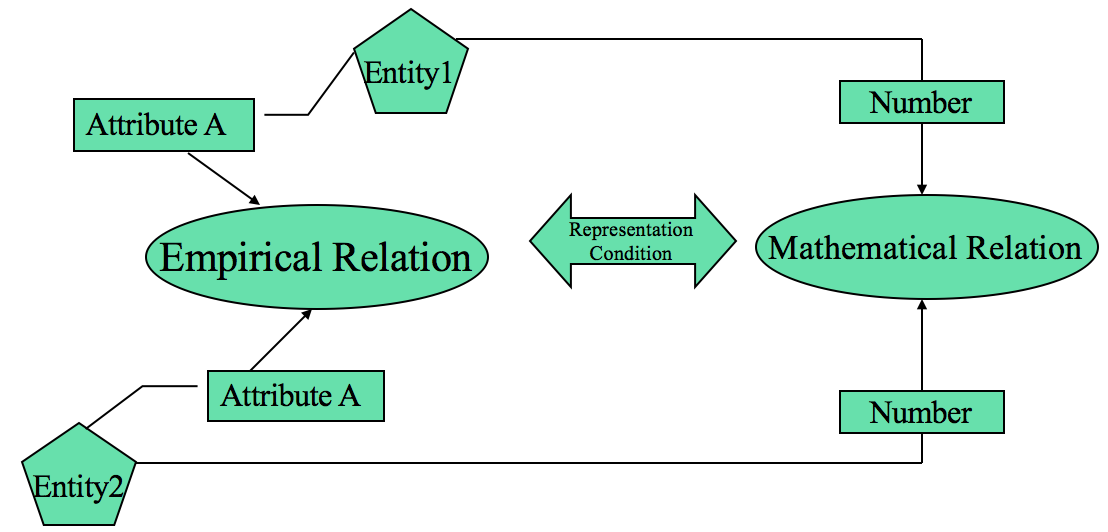
\includegraphics[width=120mm]{A2022.IDSEPC.SperimentazioneDeduzione/img-img07.png}
\end{center}
\end{frame}
%=============================================

%---------------------------------------------
\begin{frame}{\centerline{Empirical Relations}}
4

\begin{itemize}
\item  Links two entities by means of an attribute - e.g., Person (entity class) and height (attribute)
\item  Can be ambiguous - e.g., colour as perceived by human eye varies depending on subject measuring it
\item  Improves with the understanding of the attribute, and measures can foster improvement

\end{itemize}

\end{frame}
%=============================================

%---------------------------------------------
\begin{frame}{\centerline{Empirical Relations for the Attribute Height
}}
5

\begin{center}
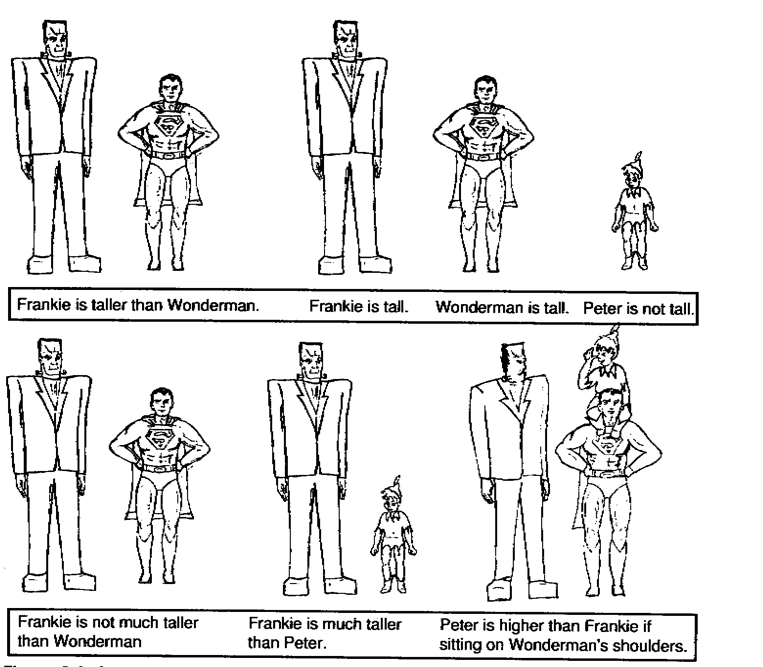
\includegraphics[width=80mm]{A2022.IDSEPC.SperimentazioneDeduzione/img-img08.png}
\end{center}

\end{frame}
%=============================================

%---------------------------------------------
\begin{frame}{\centerline{Measurement}}
6

To overcome these differences it is important to agree on:

\begin{itemize}
\item  A \textbf{measurement} is a mapping from the empirical world to the formal, relational world
\item  A \textbf{measure} is the number or symbol assignment to an entity by this mapping in order to characterise an attribute
\end{itemize}

\begin{flushright}
Fenton and Pfleeger, 1997
\end{flushright}

\end{frame}
%=============================================

%---------------------------------------------
\begin{frame}{\centerline{Measurement}}
7
\begin{center}
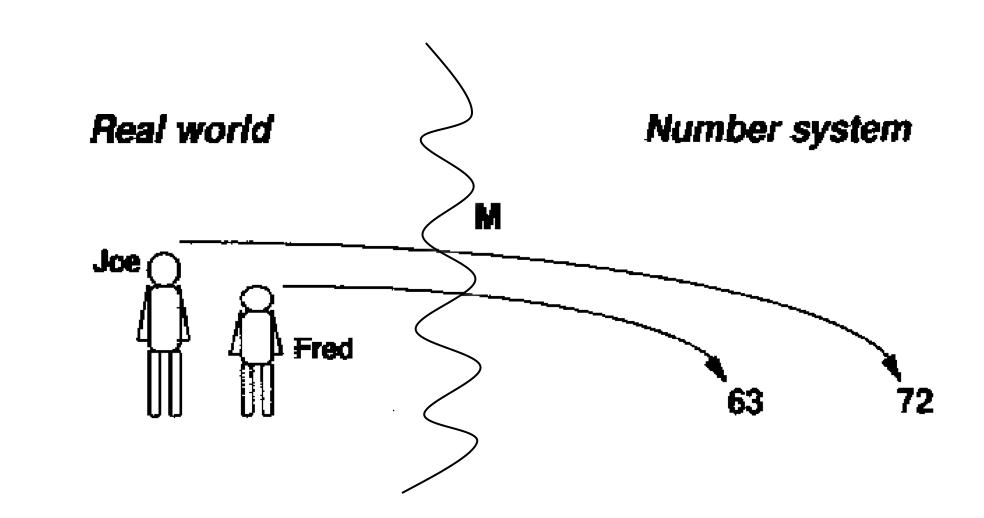
\includegraphics[width=100mm]{A2022.IDSEPC.SperimentazioneDeduzione/img-img09.png}
\newline
\end{center}

\begin{small}
\begin{center}
from Fenton pg 31
\end{center}
\end{small}

\end{frame}
%=============================================

%---------------------------------------------
\begin{frame}{\centerline{Representation Condition}}
8

\begin{itemize}
\item  A measurement mapping must map entities into numbers and empirical relation into numerical relations that preserve them and vice-versa
\end{itemize}
\begin{flushright}
Fenton and Pfleeger, 1997
\end{flushright}
\begin{itemize}
\item  \textbf{Valid} measure: satisfying the representation condition
\end{itemize}

\end{frame}
%=============================================

%---------------------------------------------
\begin{frame}{\centerline{Representation Condition}}
9

\begin{center}
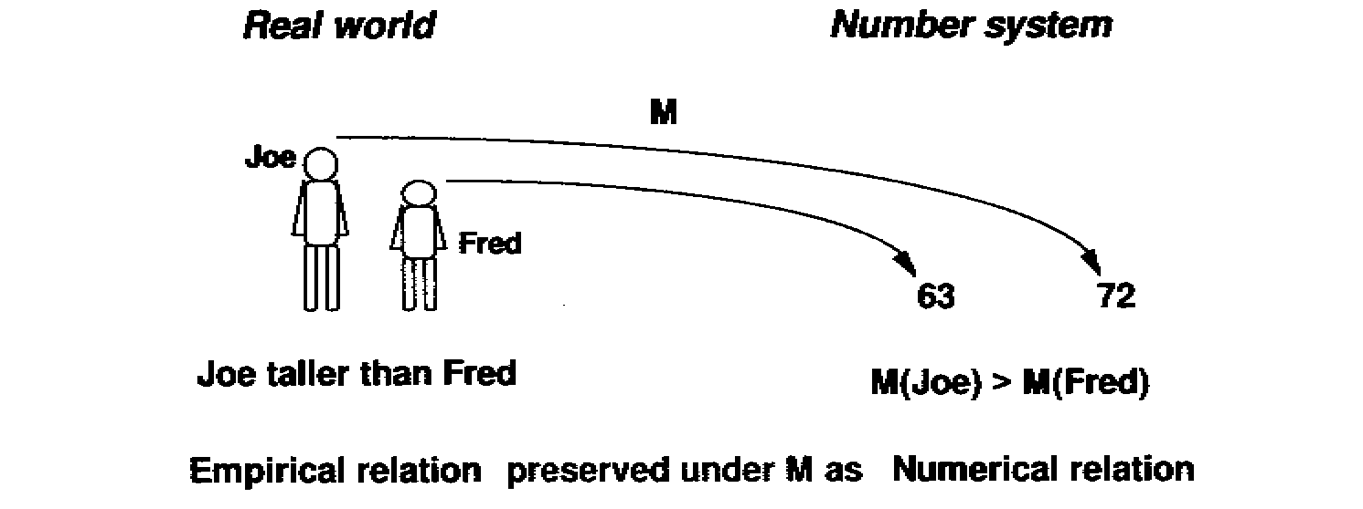
\includegraphics[width=120mm]{A2022.IDSEPC.SperimentazioneDeduzione/img-img10.png}
\newline
\end{center}

\begin{small}
\begin{center}
from Fenton pg 31
\end{center}
\end{small}

\end{frame}
%=============================================

%---------------------------------------------
\begin{frame}{\centerline{Measurement Mapping}}
0

\begin{center}
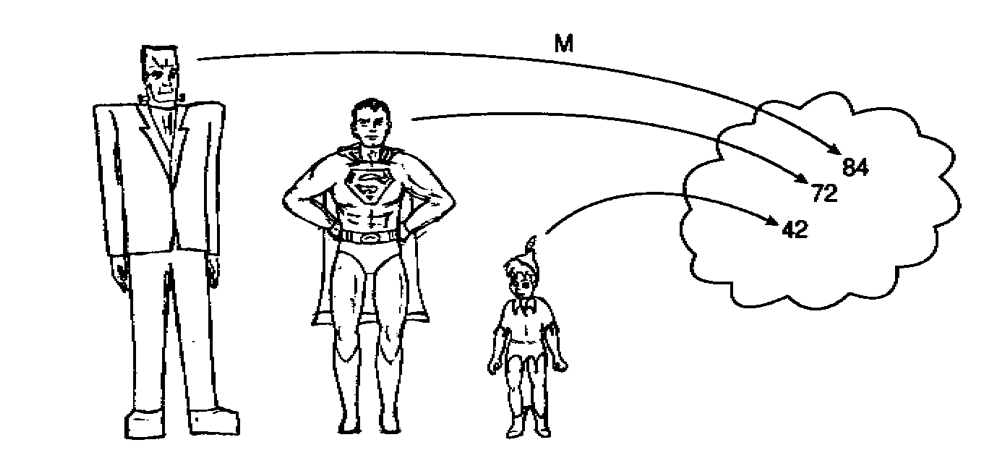
\includegraphics[width=80mm]{A2022.IDSEPC.SperimentazioneDeduzione/img-img11.png}
\begin{small}
from Fenton pg 32
\end{small}
\end{center}
\begin{table}[H]
\begin{tabulary}{\textwidth}{m{2.5cm} m{8.5cm}}
&\begin{tcolorbox}
A tall iff \(M(A) > 70\)\\
A taller than B iff \(M(A) > M(B)\)\\
A much taller than B iff \(M(A) > M(B) + 20\)
\end{tcolorbox}
\end{tabulary}
\end{table}

\end{frame}
%=============================================

%---------------------------------------------
\begin{frame}{\centerline{Role of the Representation Condition}}
1


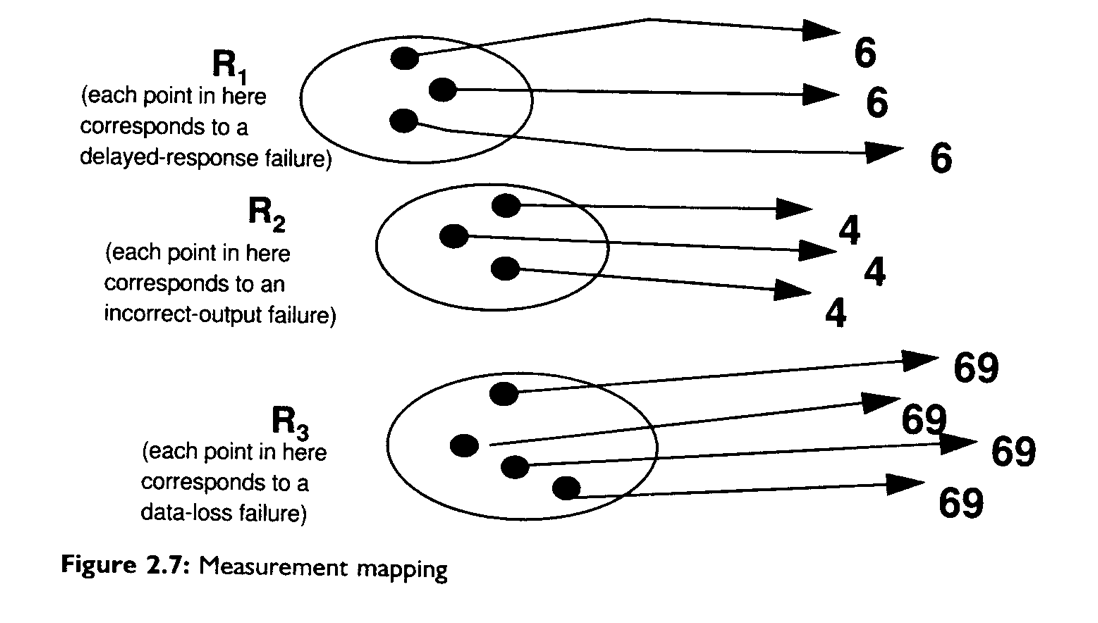
\includegraphics[width=80mm]{A2022.IDSEPC.SperimentazioneDeduzione/img-img12.png}

\begin{table}[H]
\begin{tabulary}{\textwidth}{m{7cm} m{4cm}}
\begin{small}
\begin{center}
from Fenton pg 34
\end{center}
\end{small}&
\begin{tcolorbox}
\textbf{Alternative ...}\\
\(M(R1) = 3\)\\
\(M(R2) = 4\)\\
\(M(R3) = 5\)
\end{tcolorbox}

\end{tabulary}
\end{table}


\end{frame}
%=============================================

%---------------------------------------------
\begin{frame}{\centerline{}}
2

\begin{center}
{\Large
Your Example :)
}
\end{center}


\end{frame}
%=============================================


%---------------------------------------------
\begin{frame}{\centerline{Role of the Representation Condition}}
1

\begin{itemize}
\item Beware that properly defining the representational condition in true generality is far from easy
\item Remember G\"{o}del's Disjunction$^\dag$: ``Either the human mind (even within the realm of pure mathematics) can surpass the power of any finite computing machine, or there are absolutely undecidable mathematical problems''
\end{itemize}

$^\dag$ \textit{\small
Panu Raatikainen (2018) G\"{o}del's Disjunction: The Scope and Limits of Mathematical Knowledge, History and Philosophy of Logic, DOI: 10.1080/01445340.2018.1495851}
%=============================================

\end{frame}

%---------------------------------------------
\begin{frame}{\centerline{On the Representation Condition (1/2)}}
1

\begin{itemize}
\item The program started as a philosophical problem more than a century ago:
\begin{itemize}
\item H. von Helmholtz, Zur Geschichte des Princips der kleinsten Action. Sitzungsberichte der K\"{o}niglich Preussischen Akademie der Wissenschaften zu Berlin 14, 1887
\item O. H\"{o}lder, Die Axiome der Quantit\"{a}t und die Lehre vom Mass, Berichte \"{u}ber die Verhandlungen der K\"{o}nigliche Sachsischen Gesellschaft der Wissenschaften zu Leipzig, Matematisch-Physische Klasse 53, 1 -- 64, 1901
\end{itemize}
\item It has then evolved in a economical and mathematical problem:
\begin{itemize}
\item R.D. Luce, Semiorders and a Theory of Utility Discrimination, Econometrica 24, 178 -- 191, 1956
\item L. Fuchs, Partially Ordered Algebraic Systems, Addison Wesley, Reading, Massachusetts, 1963
\item D. Krantz, Extensive Measurement in Semiorders, Philosophy of Science 34, 348 -- 62, 1967
\end{itemize}
\end{itemize}

%=============================================

\end{frame}

%---------------------------------------------
\begin{frame}{\centerline{ On the Representation Condition (2/2)}}
1

\begin{itemize}
\item After, it has been considered in social sciences: 
\begin{itemize}
\item E.W. Holman, Strong and Weak Extensive Measurement, Journal of Mathematical Psychology 6, 286 -- 293, 1969
\item A. Rutland, Measuring the zone of proximal development : studies of map-use in children with learning difficulties, PhD Dissertation, University of Stirling, 1993
\item F. Sani, J. Todman, Experimental Design and Statistics for Psychology: A First Course, John Wiley \& Sons, Apr 15, 2008 
\end{itemize}
\item Fenton adopted it in Software Engineering more as a reference than as a full theory only much later
\end{itemize}

%=============================================

\end{frame}



%---------------------------------------------
\begin{frame}{\centerline{Key Stages of Formal Measurement}}
3
\begin{center}
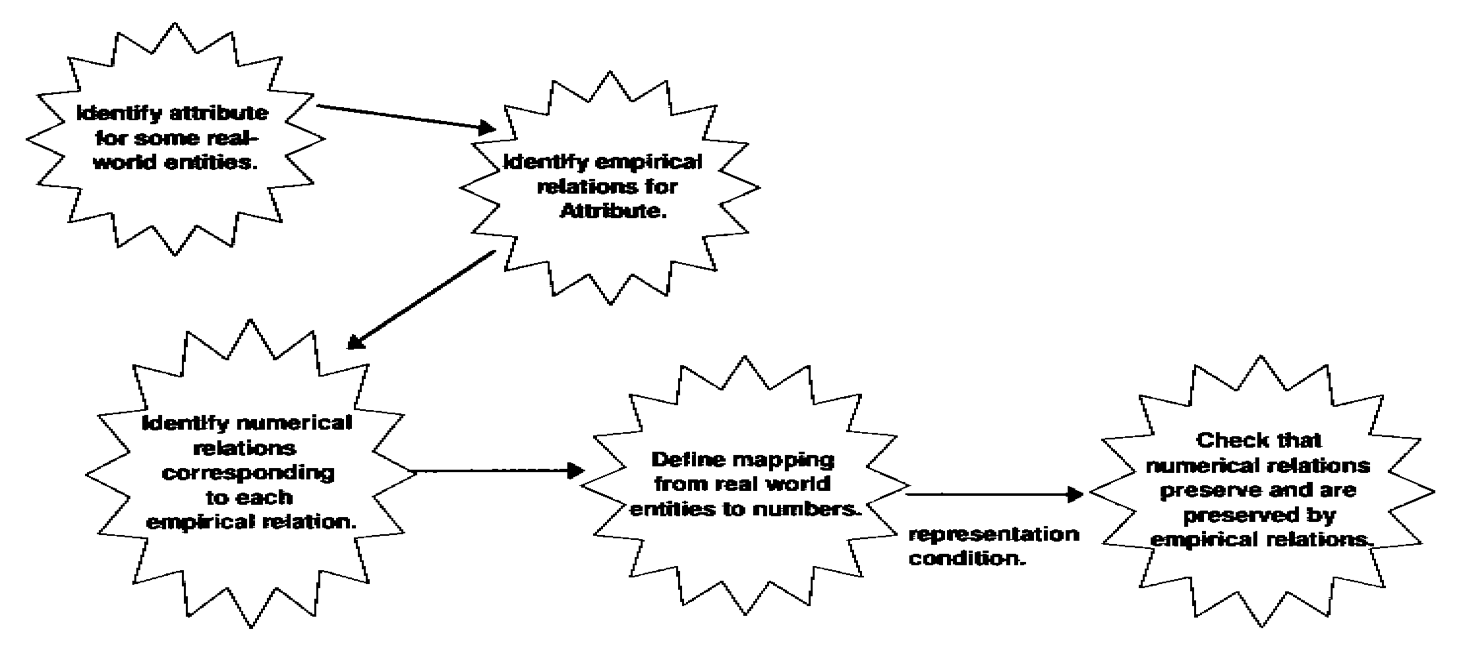
\includegraphics[width=120mm]{A2022.IDSEPC.SperimentazioneDeduzione/img-img13.png}
\newline
\end{center}

\begin{small}
\begin{center}
from Fenton pg 33
\end{center}
\end{small}
\end{frame}
%=============================================

%---------------------------------------------
\begin{frame}{\centerline{}}
2

\begin{center}
{\Large
Questions ?
}
\end{center}


\end{frame}

\begin{frame}{\centerline{Measuring progress in the work}}

\begin{center}
{\Large
Connecting measures in GQM
}
\end{center}
\end{frame}

%---------------------------------------------
\begin{frame}{\centerline{GQM approach}}


\textbf{What Should We Measure?}
\newline 

To answer this question we should answer the next questions:

\begin{itemize}
\item  What we want to study?   \textbf{Goal}
\item  How we want to study it? \textbf{Question}
\item   What should we measure? \textbf{Metrics}
\end{itemize}







\end{frame}
%=============================================

%---------------------------------------------
\begin{frame}{\centerline{GQM approach}}


The GQM is is defined on three levels:
\begin{itemize}

\item  Conceptual level (goal)
\item  Operational level (question)
\item  Quantitative level (metric)

\end{itemize}

\begin{center}
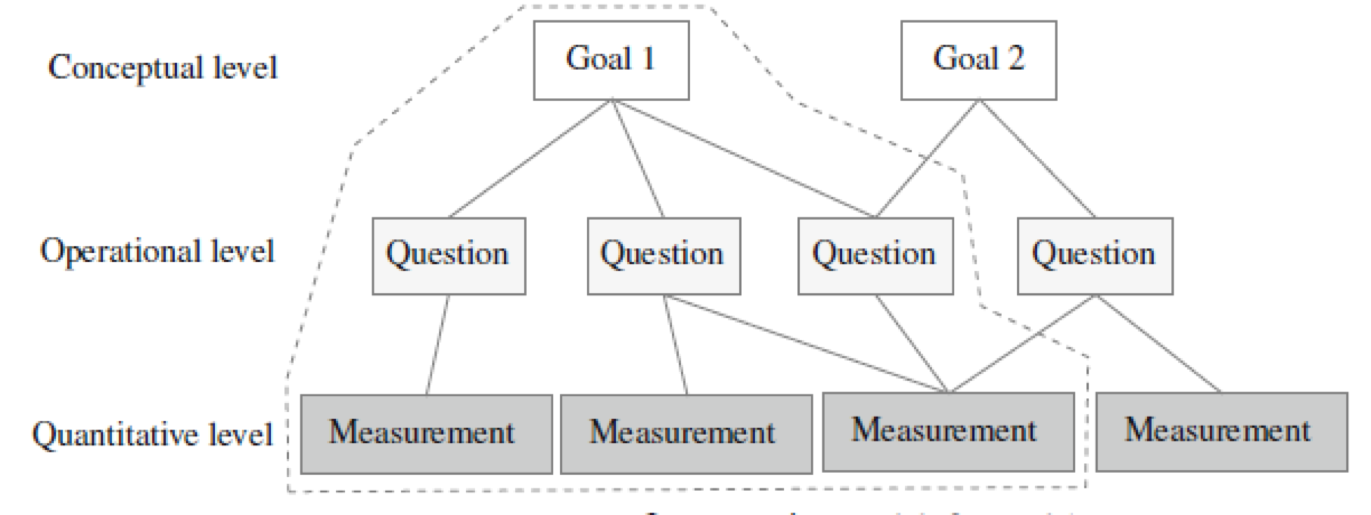
\includegraphics[width=100mm]{A2022.IDSEPC.SperimentazioneDeduzione/image-02.png}
\end{center}
\end{frame}
%=============================================

%---------------------------------------------
\begin{frame}{\centerline{Example}}


\begin{center}
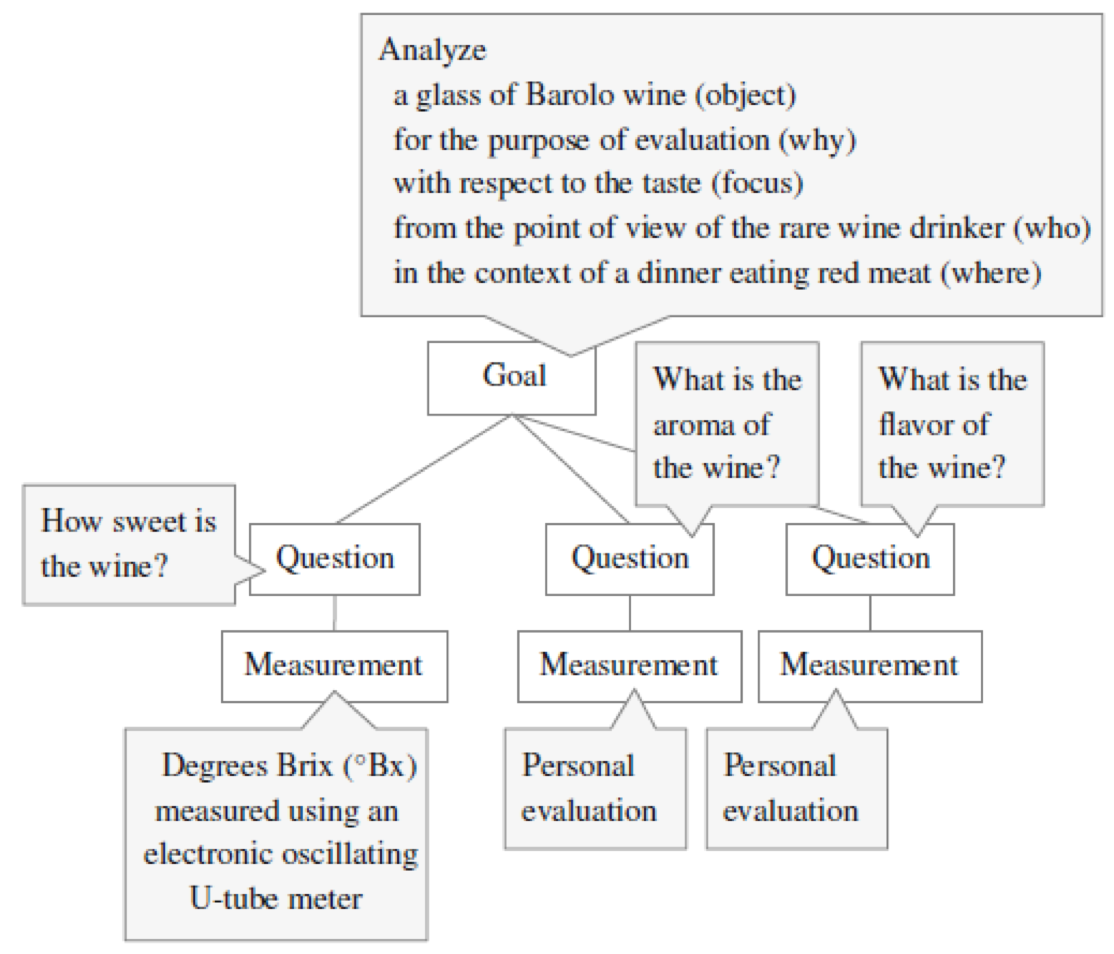
\includegraphics[width=80mm]{A2022.IDSEPC.SperimentazioneDeduzione/image-03.png}
\end{center}

\end{frame}
%=============================================

%---------------------------------------------
\begin{frame}{\centerline{Example Cont.}}


The definition of measurement goals is critical to the successful application of the GQM approach. To ease the definition of measurement goals, the GQM supplies goal templates
\begin{center}
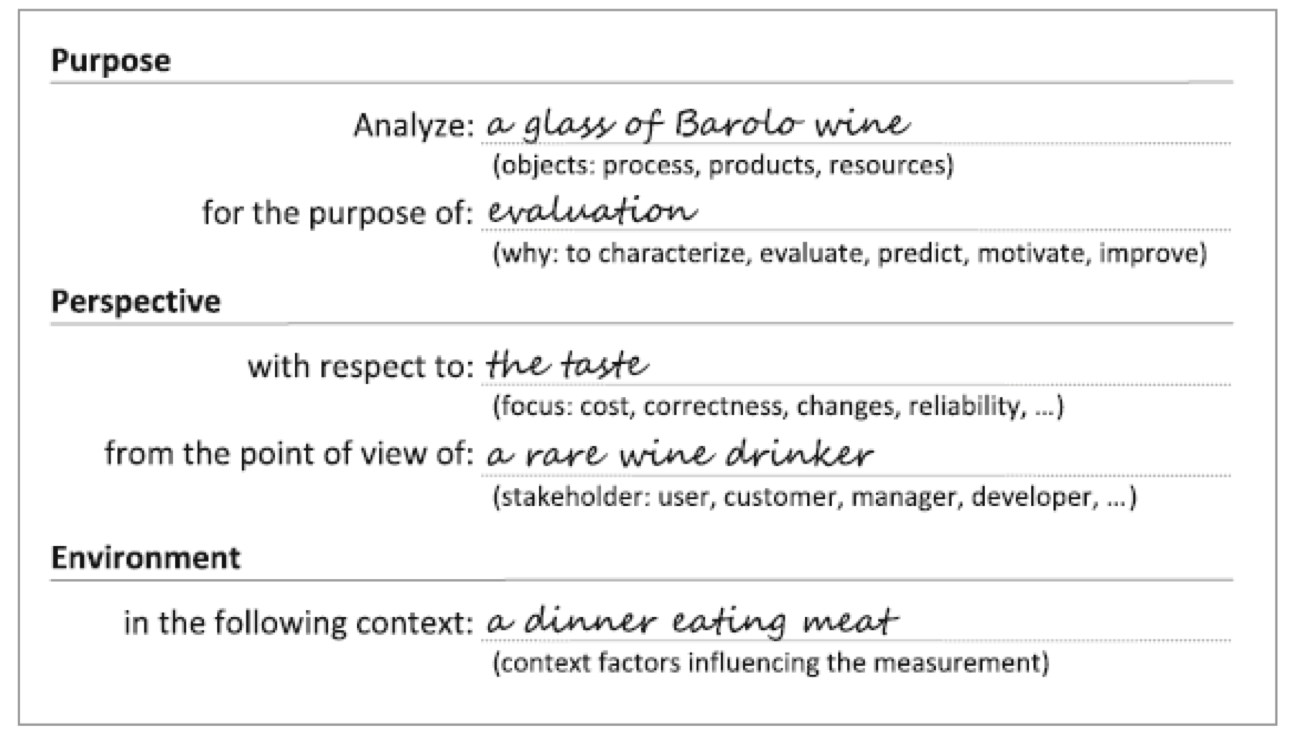
\includegraphics[width=90mm]{A2022.IDSEPC.SperimentazioneDeduzione/image-04.png}
\end{center}
\end{frame}
%=============================================

%---------------------------------------------
\begin{frame}{\centerline{Example Cont.}}
0

\begin{center}
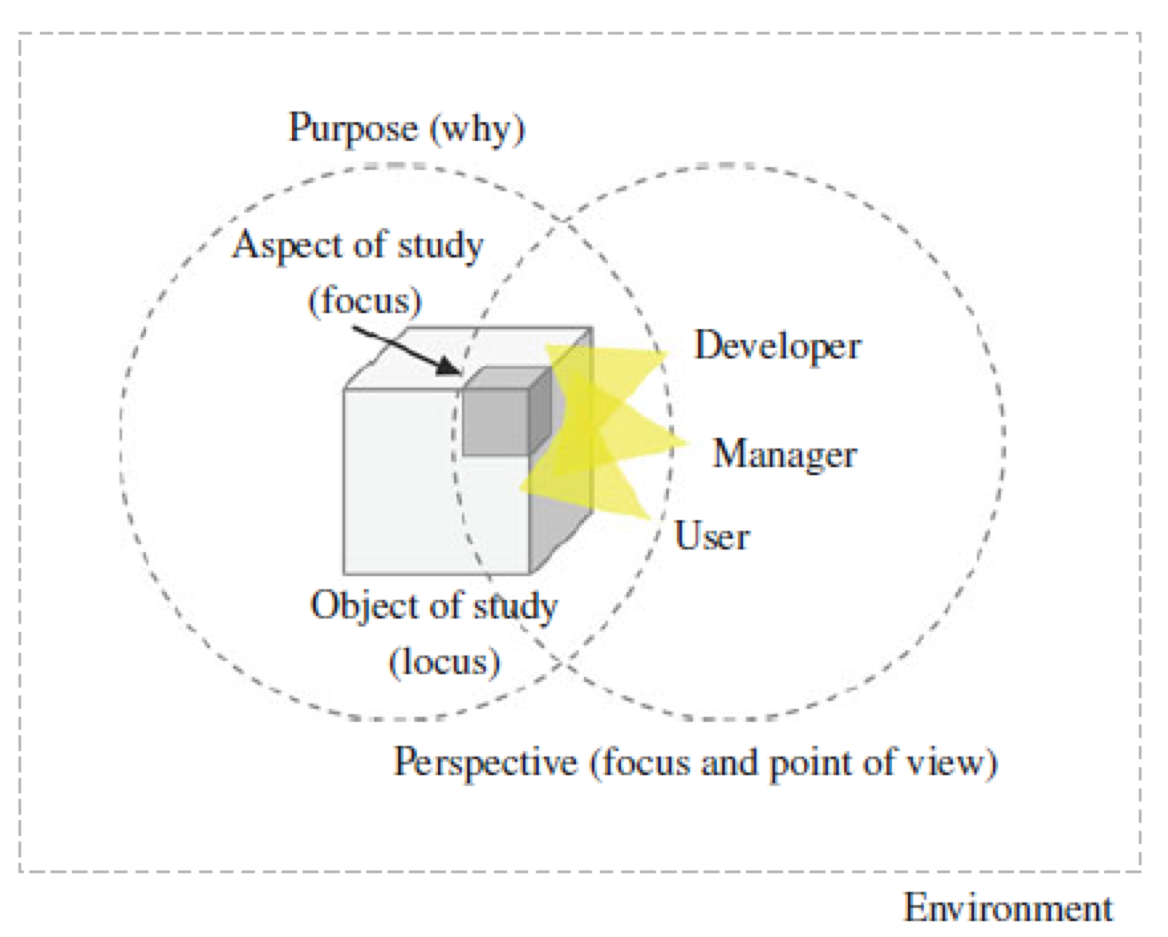
\includegraphics[width=90mm]{A2022.IDSEPC.SperimentazioneDeduzione/image-05.png}
\end{center}
\end{frame}
%=============================================

%---------------------------------------------
\begin{frame}{\centerline{GQM+Strategies}}
1

\begin{itemize}

\item  Object: the object of study;
\item  Focus: the aspect of study;
\item  Magnitude: the desired magnitude of improvement;
\item  Time frame: the time frame for achieving the goal;
\item  Organizational scope: the scope of responsibility for achieving the goal;
\item  Constraints: constraints or conflicting goals;
\item  Relationships: relationships to other goals.

\end{itemize}




\end{frame}
%=============================================

%---------------------------------------------
\begin{frame}{\centerline{GQM+Strategies}}
2

\begin{center}
business goal example

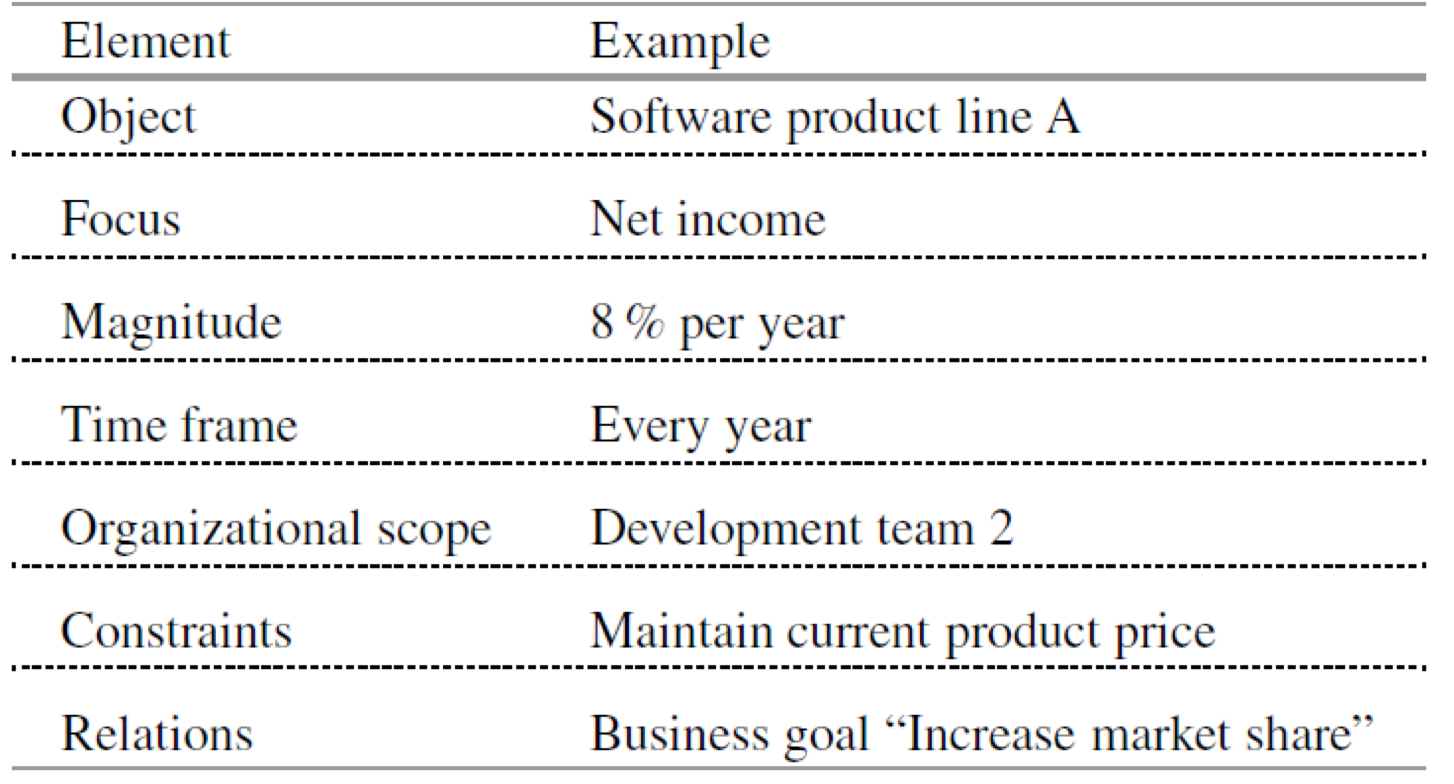
\includegraphics[width=110mm]{A2022.IDSEPC.SperimentazioneDeduzione/image-06.png}
\end{center}

\end{frame}
%=============================================

%---------------------------------------------
\begin{frame}{\centerline{GQM approach}}


\begin{center}
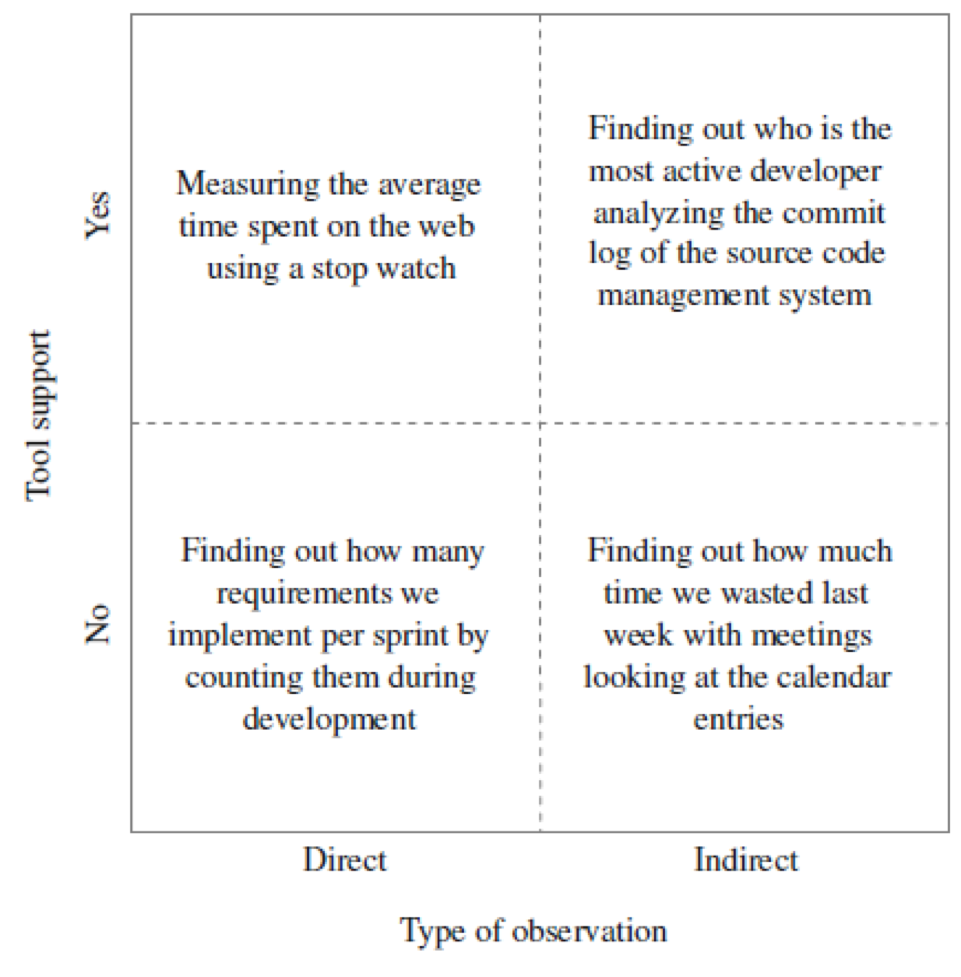
\includegraphics[width=70mm]{A2022.IDSEPC.SperimentazioneDeduzione/image-01.png}
\end{center}
\end{frame}
%=============================================
%---------------------------------------------
\begin{frame}{\centerline{SWOT analysis}}
3

\begin{itemize}

\item  Strengths: organizational aspects that support the achievement of the objective;
\item  Weaknesses: organizational aspects that inhibit the achievement of the objective;
\item  Opportunities: external conditions that support the achievement of the objective;
\item  Threats: external conditions that inhibit the achievement of the objective.


\end{itemize}

\end{frame}
%=============================================

%---------------------------------------------
\begin{frame}{\centerline{SWOT analysis}}
4

\begin{center}
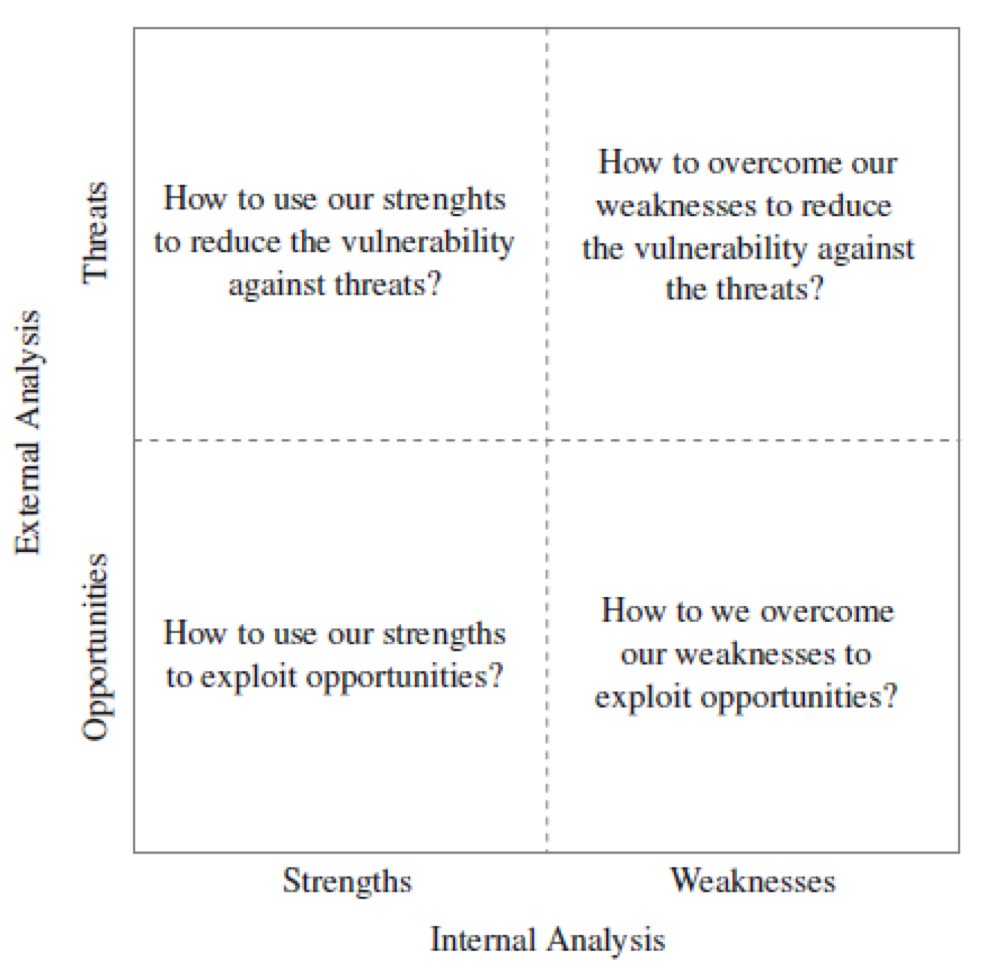
\includegraphics[width=70mm]{A2022.IDSEPC.SperimentazioneDeduzione/image-07.png}
\end{center}
\end{frame}



\begin{frame}
{\centerline{Question}}

\begin{itemize}
\item Empirical Methods are about identifying empirically laws that govern the (mutual) behaviour of entities
\item How can we perform such empirical evaluation?
\item People typically say $\ldots$ ``Experiment!!''
\item Indeed, experiments need to be properly organized in terms of GQM
\item But, as a starting point, let's see the result of experimentations...
\end{itemize}


\end{frame}

\begin{frame}
{\centerline{Galileo}}

\begin{center}
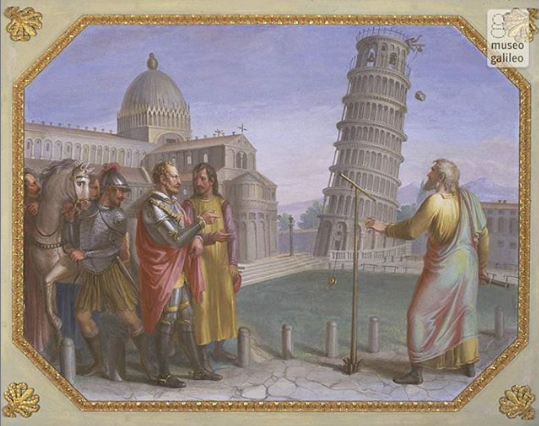
\includegraphics[width=7cm]{A2022.IDSEPC.SperimentazioneDeduzione/Galileo.png}
\end{center} 

\end{frame}


\begin{frame}
{\centerline{What about this?}}

\begin{center}
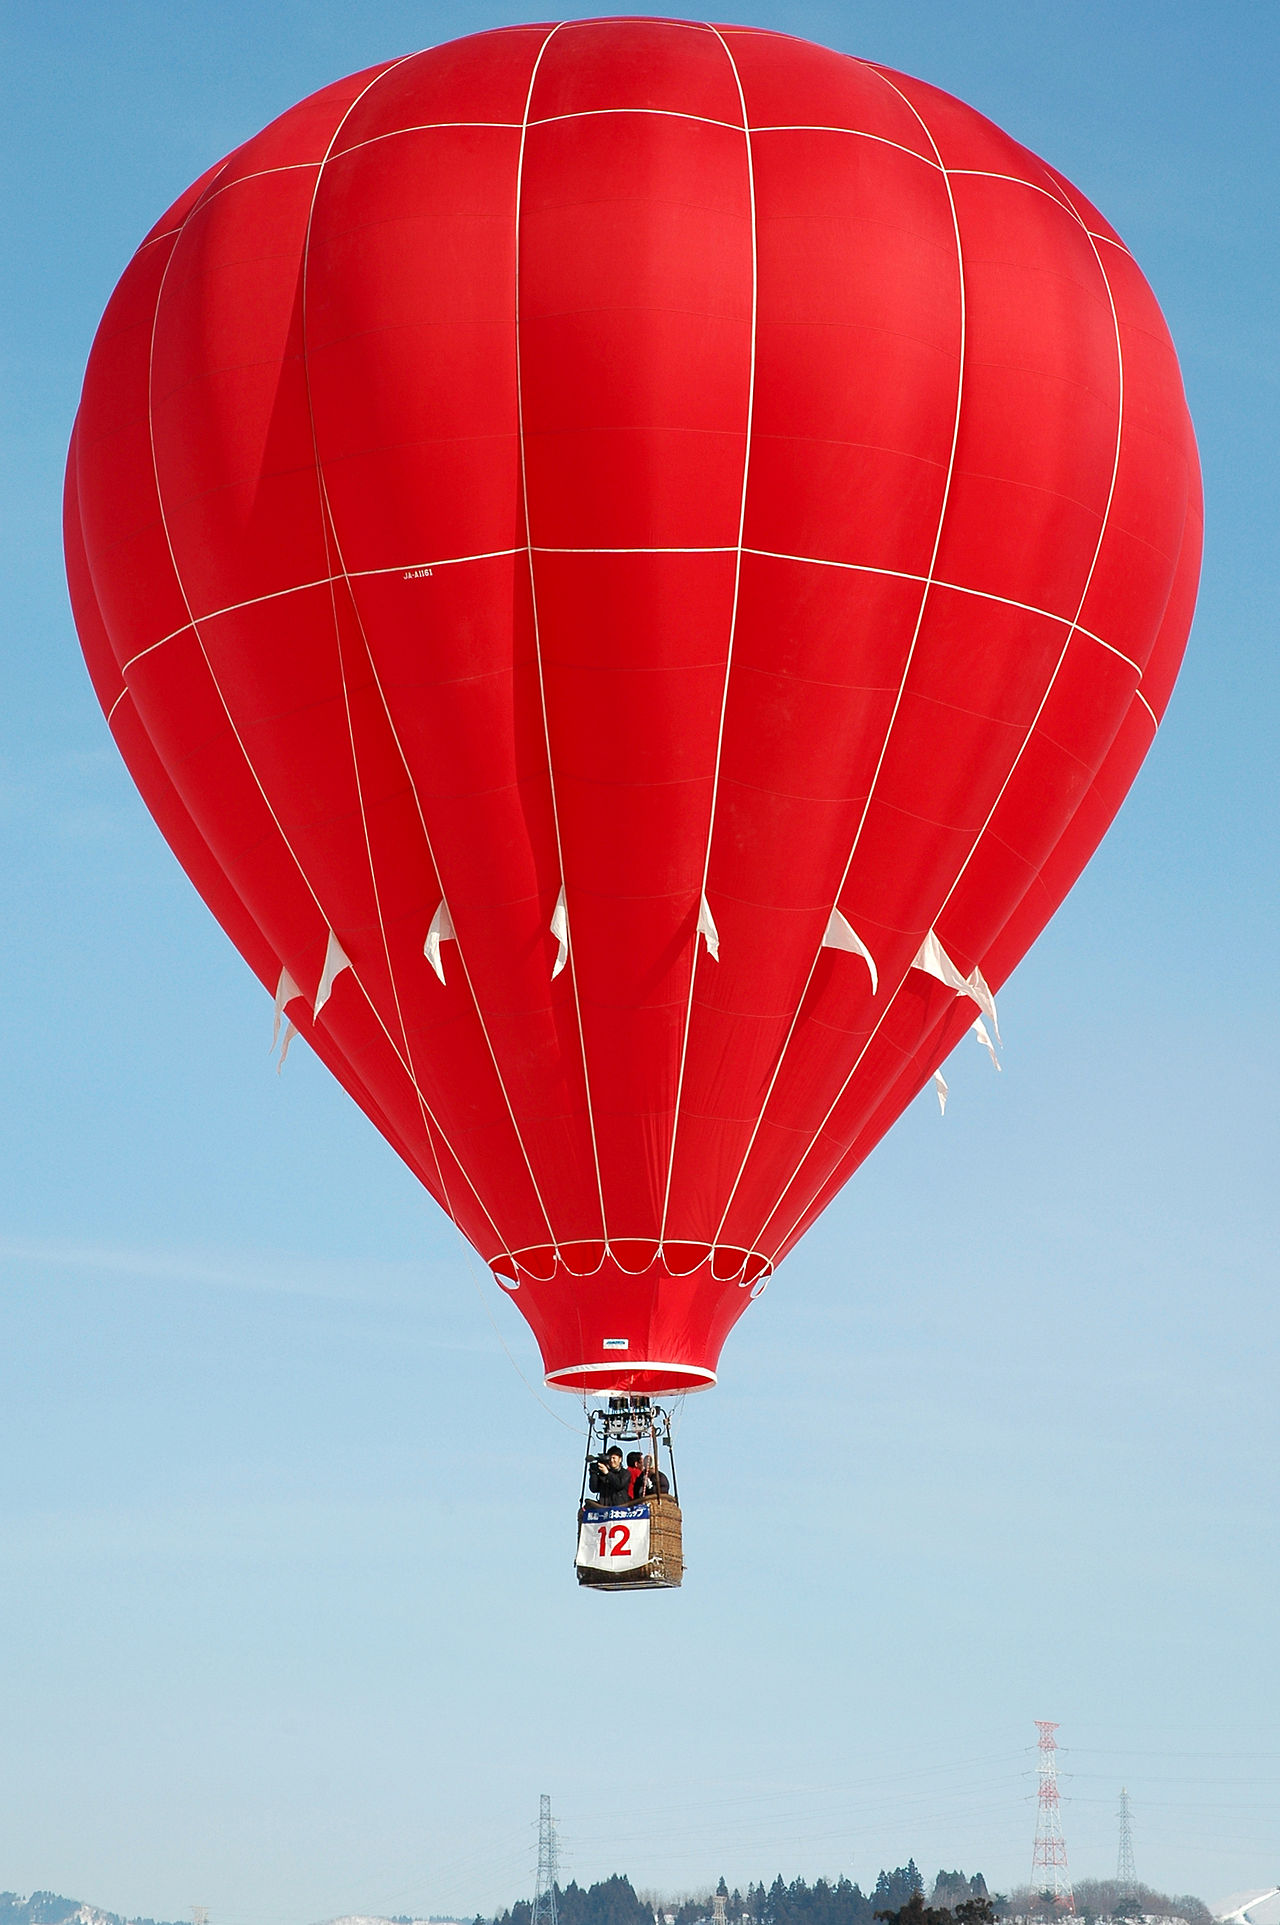
\includegraphics[width=4cm]{A2022.IDSEPC.SperimentazioneDeduzione/Mongolfiera.jpg}
\end{center} 

\begin{center}
\tiny
Source with modifications:\\
\url{https://it.wikipedia.org/wiki/Aerostato\#/media/File:2006_Ojiya_balloon_festival_011.jpg}
\end{center} 

\end{frame}

\begin{frame}
{\centerline{Interesting experimentations (for us)...}}

\begin{itemize}
\item Are agile methods more effective than traditional methods?
\item Are open source system more secure than closed source systems?
\item Is Python easier to learn than \LaTeX?
\item Are formal methods effective in reducing uncertainty?
\end{itemize}

\end{frame}

\begin{frame}
{\centerline{Answers}}

\begin{center}
\Large
\textcolor{cyan}{\bf We have no answer!}
\end{center}
\begin{itemize}
\item We need to shape better the empirical question that we want to address:
\begin{itemize}
\item With the GQM, to define with some degree of precision what we want to determine
\item Inside the GQM with Hypothesis Testing, to formulate properly the \textcolor{red}{object} of study, the \textcolor{red}{focus}  of our experiment
\item With Experimental Design, to properly consider all factors that emerged initally (and partially) while defining the GQM
\item With Statistics, to compute the result of testing the hypotheses within the defined design of the experiment.
\end{itemize}

\item We start with a \textcolor{orange}{sweet and soft} introduction to statistics
\end{itemize}

\end{frame}



\begin{frame}
{\centerline{Descriptive and Inferential Statistics (1/2)}}

\begin{itemize}
\item  \textbf{Descriptive statistics} enables us to present the data in a more meaningful way, which allows simpler interpretation of the data.
\item \textbf{Inferential statistics} are techniques that allow us to use samples to make generalizations about the populations from which the samples were drawn. It is, therefore, important that the sample accurately represents the population.
\end{itemize}


\end{frame}

\begin{frame}
{\centerline{Descriptive and Inferential Statistics (2/2)}}

Examples of tools that we use in descriptive statistics are:
\begin{itemize}
\item Measures of central tendency:
\begin{itemize}
\item the mean,
\item the median, 
\item the mode,
\item $\ldots{}$
\end{itemize}
\item Measures of spread:
\begin{itemize}
\item the variance,
\item the range,
\item the 95-percentile,
\item $\ldots{}$
\end{itemize}
\end{itemize}

\end{frame}

%----------------------------------------------------------------------------------------

%------------------------------------------------
\begin{frame}
{\centerline{Statistical concepts -- Population}}
\textbf{Population} -- set of objects that are studied in a task.



\begin{center}

\includegraphics[width=8cm]{A2022.IDSEPC.SperimentazioneDeduzione/pop-1.png}
\end{center} 

\end{frame}

%----------------------------------------------------------------------------------------


%------------------------------------------------
\begin{frame}
{\centerline{Statistical concepts -- Sample}}


\textbf{Sample} -- finite set of objects from the population.

\begin{center}

\includegraphics[width=8cm]{A2022.IDSEPC.SperimentazioneDeduzione/sam-1.png}
\end{center} 

\end{frame}

%----------------------------------------------------------------------------------------

%------------------------------------------------
\begin{frame}
{\centerline{Statistical concepts }}

Samples maybe different...

\begin{center}
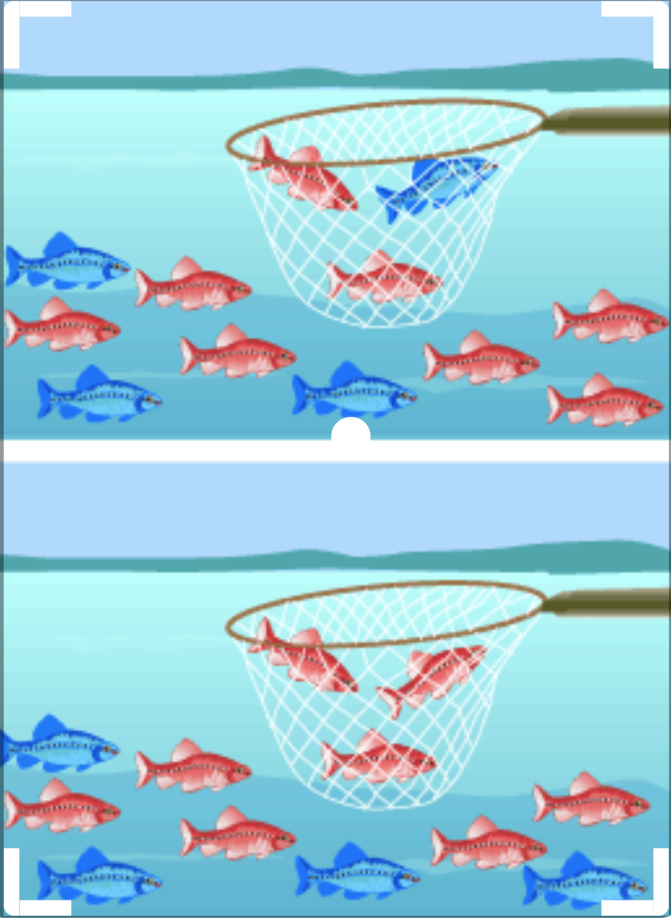
\includegraphics[width=3cm]{A2022.IDSEPC.SperimentazioneDeduzione/fish-pop.png}
\end{center} 

But sample should represent main properties of population (that are investigated in the research / analysis )

Reliable statistical analysis requires  \textcolor{red}{\bf representative samples}.
\end{frame}

%----------------------------------------------------------------------------------------




%------------------------------------------------
\begin{frame}
{\centerline{Statistical concepts -- Sample Size}}

$$X^n = (X_1, \ldots, X_n).$$
\centering
n -- sample size


\begin{center}
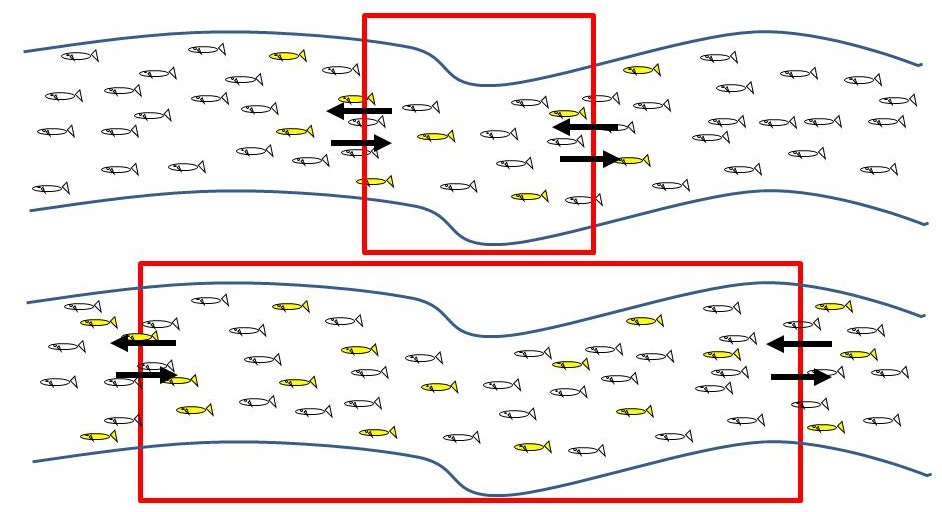
\includegraphics[width=8cm]{A2022.IDSEPC.SperimentazioneDeduzione/figure2_mrc.jpg}
\end{center} 

\end{frame}

%----------------------------------------------------------------------------------------



%------------------------------------------------
\begin{frame}
{\centerline{Statistical concepts -- Simple sample}}

$X^n - $ \textbf{simple sample}, if $X_1,\ldots, X_n$ - independently identically distributed (i.i.d.) random variables. Each has the same density function $f(x)$.


\end{frame}

%----------------------------------------------------------------------------------------




\begin{frame}
{\centerline{Statistical concepts (1/4)}}

A statistic $T(X^n)$ -- is a function of a sample. 
\newline


\textbf{For the central tendency,} 

\begin{itemize}
\item Let $X$ be our sample:
$$X = \{ X_1 \ldots{} X_n \}$$
\begin{itemize}
\item E.g.,  $X = \{ 1, 2, 4, 4, 4, 2, 0, 9, 0, 1 \}$
\end{itemize}

\item \textcolor{red}{Notice that we write it as a set, but it is a bag and not a set, since there can be duplicates. }


\end{itemize}

\end{frame}

\begin{frame}
{\centerline{Statistical concepts (2/4)}}

\begin{itemize}
\item Sample mean:
$$ \bar{X} = \frac{1}{n}\sum_{i=1}^{n}X_i$$ 
\begin{itemize}
\item In our case it is 2.7
\end{itemize}
\vspace*{0.5cm}
\item Sample median:
$$  median(X) = X_j : X_j \text{~ is central} $$ 
\begin{itemize}
\item In our case it is 2
\end{itemize}


\end{itemize}

\end{frame}

\begin{frame}
{\centerline{Statistical concepts (3/4)}}

\begin{itemize}
\item Sample median more formally \textcolor{red}{\em (Is it useful? -- we need to experiment it $\ldots{}$)}:\\

\begin{equation*}
\begin{split}
median(X) = X_j   :  abs( & card(\{X_k : X_k \in X, X_k \le X_j\}) -  \\
                                       &  card(\{X_h : X_h \in X, X_h \ge X_j\})) \le 1
\end{split}
\end{equation*}

\item Sample mode:
$$  mode(X) = X_j : X_j \text{ is the most frequent value in } X$$ 
\begin{itemize}
\item In our case it is 4
\end{itemize}


\end{itemize}


\end{frame}

\begin{frame}
{\centerline{Statistical concepts (4/4)}}

\begin{itemize}

\item Sample mode more formally:

$$  mode(X) = \argmax_{x \in X} (occurrences(x,X))$$ 

where:
$$ occurrences(a,S) = \text{ number of elements of a } \in S $$



\end{itemize}


\end{frame}




\begin{frame}
{\centerline{Definition of statistic}}

A statistic $T(X^n)$ -- is a function of a sample. 
\newline


\begin{itemize}

\item We have seen the sample mean:
$$ \bar{X} = \frac{1}{n}\sum_{i=1}^{n}X_i$$ 
\newline

\item We can have the sample variance:
$$ S^2_n = \frac{1}{n}\sum_{i=1}^{n}(X-\bar{X})^2$$
\begin{itemize}
\item In our case it is 66.1
\end{itemize}
\end{itemize}

\end{frame}



%------------------------------------------------
\begin{frame}
{\centerline{Back on kinds of statistics (1/2)}}


\begin{center}

 \textcolor{cyan}{{\it To remember \#1:} \textbf{Descriptive statistics computes} properties of the sample, the sample statistics.}
 
 \vspace*{1cm}

 \textcolor{orange}{{\it To remember \#2:} \textbf{Inferential statistics estimates}  the population parameters from the sample statistics.}

 \vspace*{1cm}

\textcolor{red}{{\it To remember \#3:}  \textcolor{cyan}{Statistics are computed,}  \textcolor{orange}{parameters are estimated}.}
\end{center}


\end{frame}

\begin{frame}
{\centerline{Back on kinds of statistics (2/2)}}

\begin{itemize}
\item Any time we move from sample to population we perform estimations,
\begin{itemize}
\item i.e., we use statistics to estimate parameters of the population, and different statistics have different properties
\end{itemize}
\item Estimations have properties and need to be as \textit{precise} as possible.
\end{itemize}

\end{frame}

%------------------------------------------------
\begin{frame}
{\centerline{Estimations}}

A good estimator must satisfy three conditions:
\begin{itemize}
\item \textcolor{blue}{Unbiased}: The expected value of the estimator must be equal to the mean of the parameter.
\item \textcolor{blue}{Consistent}: The value of the estimator approaches the value of the parameter as the sample size increases.
\item \textcolor{blue}{Relatively Efficient}: The estimator has the smallest variance of all estimators which could be used.
\end{itemize}
\end{frame}


\begin{frame}
{\centerline{Estimates and point estimates}}


\begin{itemize}
\item We have two kinds of estimates:
\begin{itemize}
\item Point estimates
\item Interval estimates
\end{itemize}
\item A point estimate is the single best guess about the value of parameter.
\end{itemize}

\end{frame}

%----------------------------------------------------------------------------------------

%------------------------------------------------

%----------------------------------------------------------------------------------------

%------------------------------------------------

\begin{frame}
{\centerline{Interval estimates}}

\begin{itemize}
\item An \textcolor{red}{interval estimate} is an interval that contain the true value of the corresponding parameter with the specified probability.
\item It is also called the \textcolor{blue}{confidence interval}.
\item \textit{We will see later that if the distribution of a random variable Z is Normal (N(0,1)), then:}
\end{itemize}

$$\mathbb{P} (-z_r\leq Z \leq z_r) = r$$

\begin{center}
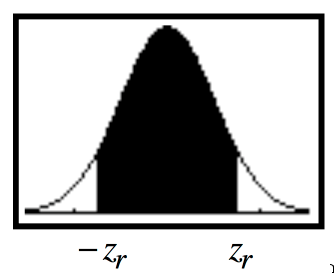
\includegraphics[width=2.5cm]{A2022.IDSEPC.SperimentazioneDeduzione/conf-int-ex-1.png}
\end{center} 
Where:

\begin{itemize}
\item $z_r$ - z-score
\item $r$ - level of confidence (usually, denoted as $1-\alpha$)
\end{itemize}
\end{frame}


\begin{frame}
{\centerline{Unbiased estimator}}


Any statistic whose mathematical expectation is equal to a parameter $\theta$ is called an \textbf{unbiased estimator} of the parameter $\theta$. Otherwise, the statistic is said to be \textbf{biased}.

\end{frame}
%------------------------------------------------


\begin{frame}
{\centerline{Bias of an estimator}}


The \textbf{bias} of an estimator $\hat{\theta_n}$ is 

$$\mathbb{E}(\hat{\theta}) - \theta $$ 


\end{frame}
%------------------------------------------------



\begin{frame}
{\centerline{Bias-variance decomposition}}


\begin{itemize}
\item  The mean squared error MSE is:
 $$MSE = \mathbb{E}(\hat{\theta} - \theta)^2$$. 

\item The \textbf{bias-variance decomposition} for the MSE of an estimator $\hat{\theta_n}$
$$MSE = bias^2(\hat{\theta_n}) + \text{Var}(\hat{\theta_n})$$.

\item We will prove this formula later in the course.
\end{itemize}

\end{frame}
%------------------------------------------------


\begin{frame}
{\centerline{Hypothesis testing}}

\begin{itemize}
\item Now we introduce the following concepts:

\begin{itemize}
\item (a) A statistical hypothesis.
\item (b) A test of a hypothesis against an alternative hypothesis and the associated concept of the critical region of the test.
\item (c) The power of a test.
\end{itemize}
\end{itemize}

\end{frame}


\begin{frame}
% Cluttered !!!
{\centerline{Example}}

\begin{itemize}
\item Let $X$ be an outcome of a random experiment, for example, some test score, $X \sim N(\theta, 100)$.
\item Some past experience says that $\theta=75$.
\item After some changes we suspect that no longer $\theta=75$, but $\theta>75$
\begin{itemize}
\item  $\theta>75$ is our \textbf{statistical hypothesis}
\end{itemize}
\item However, our hypothesis might be false, hence $\theta \leq 75$ (this also may be considered as a hypothesis). 
\begin{itemize}
\item $\theta \leq 75$  may be considered as a hypothesis
\end{itemize}

\end{itemize}




\end{frame}
%----------------------------------------------------------------------------------------




\begin{frame}
% Cluttered !!!
{\centerline{Example}}



\begin{itemize}
\item Thus, we have two hypotheses:
\begin{itemize}
\item An first hypothesis of no effect, which we represent as $H_0$, and which we call \textcolor{red}{null hypothesis}
\item Another hypothesis of a specific effect, which we represent as $H_1$, and which we call \textcolor{red}{alternate hypothesis}
\end{itemize}
\item In our case we can say:
\begin{itemize}
\item Null hypothesis:
$$H_0: \theta \leq 75$$
\item Alternate hypothesis:
$$H_1: \theta > 75$$
\end{itemize}
\end{itemize}


\end{frame}
%----------------------------------------------------------------------------------------


\begin{frame}
% Cluttered !!!
{\centerline{Example}}

\begin{itemize}
\item To check $H_0$ against $H_1$ we run the experiment 
\item We consider a random sample $X_1,\ldots, X_n$ from $N(\theta, 100)$ 
\item We devise a \textcolor{red}{test}, i.e., a rule, that will tell us what decision to make once we get observations $x_1,\ldots, x_n$.
\item For the sake of the example, we assume $n=25$.
\newline
\end{itemize}

\begin{center}
How do we construct the test -- the rule?
\end{center}

\begin{itemize}
\item This will be the subject of the last lectures of the course
\begin{itemize}
\item and the beginning of the twin course on advanced statistics
\end{itemize}
\item Now we just provide an intuitive explanation
\end{itemize}


\end{frame}

%----------------------------------------------------------------------------------------
%----------------------------------------------------------------------------------------

\begin{frame}
{\centerline{Procedure (1/2)}}

\begin{itemize}
\item We want to determine if the  alternate hypothesis $H_1$ with a \textit{negative} approach
\item We check if we can reject the null hypothesis $H_1$ with a high level of probability, say, 95\%
\item We divide the sample in two parts, one of which can also be empty. Formally speaking we say that:
\item We  partition the sample space into a subset $C$ and its complement $C^*$.
\item Let us assume that the experiments lead to outcomes  $X_1,\ldots, X_n$, which are reflected to the values $x_1,\ldots, x_n$
\end{itemize}


\end{frame}

\begin{frame}
{\centerline{Procedure (2/2)}}

\begin{itemize}
\item If the point $(x_1,\ldots, x_n) \in C$, we reject the hypothesis $H_0$, otherwise we cannot reject $H_0$. 
\item If we reject the null hypothesis, we claim that the alternate hypothesis hold.
\item If we cannot reject the null hypothesis, right now we cannot draw any conclusion.
\end{itemize}

\vspace*{1cm}
\begin{center}
$C$ is the \textcolor{red}{critical region} of the test.
\end{center}

\end{frame}


%----------------------------------------------------------------------------------------
%----------------------------------------------------------------------------------------



\begin{frame}
{\centerline{Example. Test 1 (1/2)}}
There are a lot of rules (tests). We start with \textbf{Test 1}
$$C = \{ (x_1,\ldots, x_n); (x_1 + x_2 + \ldots + x_n > 25*75) \}$$
We shall reject $H_0$ if and only if $(x_1,\ldots, x_n) \in C$.

$$\bar{x} = \frac{1}{25} \sum_{1}^{25} x_i$$

We accept $H_0: \theta \leq 75$ if $\bar{x} \leq 75$. 

\vspace*{1cm}
\begin{center}
Note: This will be all proved formally during the last lectures of of the course.
\end{center}

\end{frame}

%----------------------------------------------------------------------------------------
%------------------------------------------------

%----------------------------------------------------------------------------------------
%----------------------------------------------------------------------------------------



\begin{frame}
{\centerline{Example. Test 1 (1/2)}}

The rule: We shall \textbf{reject} the $H_0: \theta \leq 75$ if the mean of the sample \textbf{exceeds the maximum value of the mean of the distribution} when the hypothesis $H_0$ is true.
\newline 

$$\bar{X} \sim N(\theta, 100/n) = N(\theta, 100/25) = N(\theta, 4)$$

\vspace*{1cm}
\begin{center}
Note: This will be all proved formally during the last lectures of of the course.
\end{center}

\end{frame}

%----------------------------------------------------------------------------------------
%------------------------------------------------




%----------------------------------------------------------------------------------------
%------------------------------------------------


\begin{frame}
{\centerline{Hypothesis testing. Definitions}}
\textbf{Definition 1.} A \textbf{ statistical hypothesis} is an assertion about the distribution of one or more random variables. If the statistical hypothesis completely specifies the distribution, it is called a simple statistical hypothesis; if it does not, it is called a composite statistical hypothesis.

\end{frame}
%----------------------------------------------------------------------------------------

\begin{frame}
{\centerline{Hypothesis testing. Definitions}}

\textbf{Definition 2.} A test of a statistical hypothesis is a rule which, when the experimental sample values have been obtained, leads to a decision to accept or to reject the hypothesis under consideration.

\end{frame}
%----------------------------------------------------------------------------------------

%------------------------------------------------

\begin{frame}
{\centerline{Hypothesis testing. Definitions}}
\textbf{Definition 3.} Let $C$ be that subset of the sample space which, in accordance with a prescribed test, leads to the rejection of the hypothesis under consideration. Then $C$ is called \textbf{the critical region} of the test.

\begin{center}
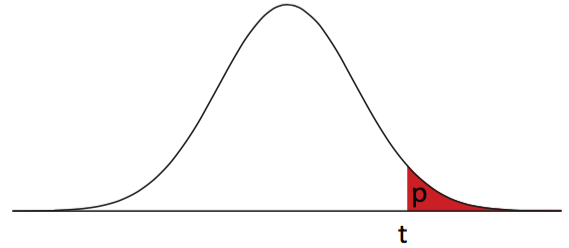
\includegraphics[width=4cm]{A2022.IDSEPC.SperimentazioneDeduzione/norm-hypo.png}
\end{center}

\end{frame}


%------------------------------------------------

\begin{frame}
{\centerline{Hypothesis testing. Definitions}}



\textbf{Definition 4.} \textbf{The p-value} associated with a test (again) is the probability that we obtain a value of the test statistic that is at least as extreme as the observed value of our test statistic assuming the $H_0$ hypothesis is true.
\end{frame}

%----------------------------------------------------------------------------------------

%------------------------------------------------

\begin{frame}
{\centerline{Hypothesis testing. Summary}}

The following 5 steps are followed when testing hypotheses:
\begin{itemize}
\item Specify $H_0$ and $H_1$ -- the null and alternative hypotheses
\item Determine the appropriate test statistic
\item Determine the critical region
\item Compute the value of the test statistic
\item Make decision
\end{itemize}

\end{frame}

%----------------------------------------------------------------------------------------

\begin{frame}
{\centerline{Errors of a test (1/2)}}

%table
\begin{center}
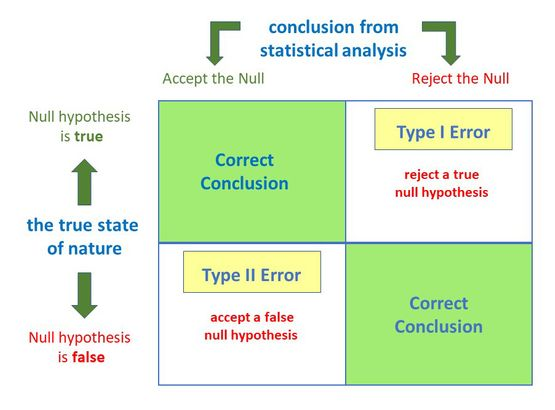
\includegraphics[width=8cm]{A2022.IDSEPC.SperimentazioneDeduzione/type-1-and-2-errors.jpg}
\end{center}

\vspace*{0.5cm}
\begin{center}
\tiny
Taken with modifications from: \url{https://www.simplypsychology.org/type_I_and_type_II_errors.html}
\end{center}

\end{frame}

\begin{frame}
{\centerline{Errors of a test (2/2)}}
There could be errors of two kind:
\begin{itemize}
\item A \textcolor{red}{type 1} error is when we reject the null hypothesis when the null hypothesis is true, that is we think that something is going on, but nothing is really there. 
\begin{itemize}
\item The probability of committing a type 1 error is typically referred to as \textcolor{orange}{$\alpha$}.
\end{itemize}

\item A \textcolor{red}{type 2} error is when we fail to reject the null hypothesis when actually we should reject it, that is, we fail to perceive a phenomena.
\begin{itemize}
\item The probability of committing a type 2 error is typically referred to as  \textcolor{orange}{$\beta$}. 
\end{itemize}
\end{itemize}


The power function of a test informally is the probability of not committing a type 2 error, that is, $(1-\beta)$

\end{frame}


\begin{frame}
{\centerline{Back to the example (1/9)}}

\begin{center}
\Large
\textcolor{cyan}{Is the Test 1 good?}
\end{center}

\vspace*{1cm}

\begin{center}
\Large
We are now going to see only a trailer.
\end{center}

\begin{itemize}
\item The full movie will be played throughout the course
\item But perceive the big picture now before progressing...

\end{itemize}

\end{frame}

\begin{frame}
{\centerline{Back to the example (2/9)}}


Let us construct \textbf{the power function} of the Test 1: $K_{1}(\theta) = \mathbb{P}(\bar{X}>75);$   $K_1(75) = 0.5.$ 
See the standard normal distribution table.
\begin{center}
  
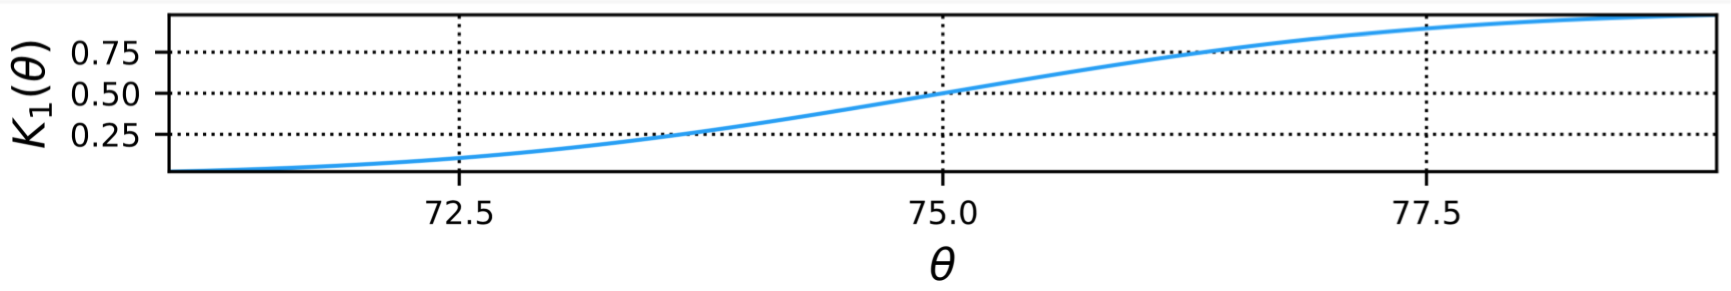
\includegraphics[width=11cm]{A2022.IDSEPC.SperimentazioneDeduzione/k1.png}
\end{center}

Is it good to reject $H_0$, when $H_0$ is true (in 50\% of cases)?

\vspace*{1cm}
\begin{center}
\textcolor{green}{\textit{Remember, this is just a trailer, you are not required to fully learn it right now $\ldots{}$}}
\end{center}

\end{frame}


%----------------------------------------------------------------------------------------
%----------------------------------------------------------------------------------------

\begin{frame}
{\centerline{Back to the example (3/9)}}
Let us try another one, Test 2:
$$C = \{ (x_1,\ldots, x_n): (x_1 + x_2 + \ldots + x_n > 25*78) \}$$
We shall reject $H_0$ if and only if $(x_1,\ldots, x_n) \in C$.

\vspace*{1.5cm}
\begin{center}
\textcolor{green}{\textit{Remember, this is just a trailer, you are not required to fully learn it right now $\ldots{}$}}
\end{center}

\end{frame}

%----------------------------------------------------------------------------------------
%----------------------------------------------------------------------------------------


\begin{frame}
{\centerline{Back to the example (4/9)}}

The power function of the Test 2: 

$$K_{2}(\theta) = \mathbb{P}(\bar{X}>78) = 1 - N\left(\frac{78-\theta}{2}\right)$$

\vspace*{1.5cm}
\begin{center}
\textcolor{green}{\textit{Remember, this is just a trailer, you are not required to fully learn it right now $\ldots{}$}}
\end{center}

\end{frame}

%----------------------------------------------------------------------------------------
%----------------------------------------------------------------------------------------


\begin{frame}
{\centerline{Back to the example (5/9)}}


\begin{center}
  
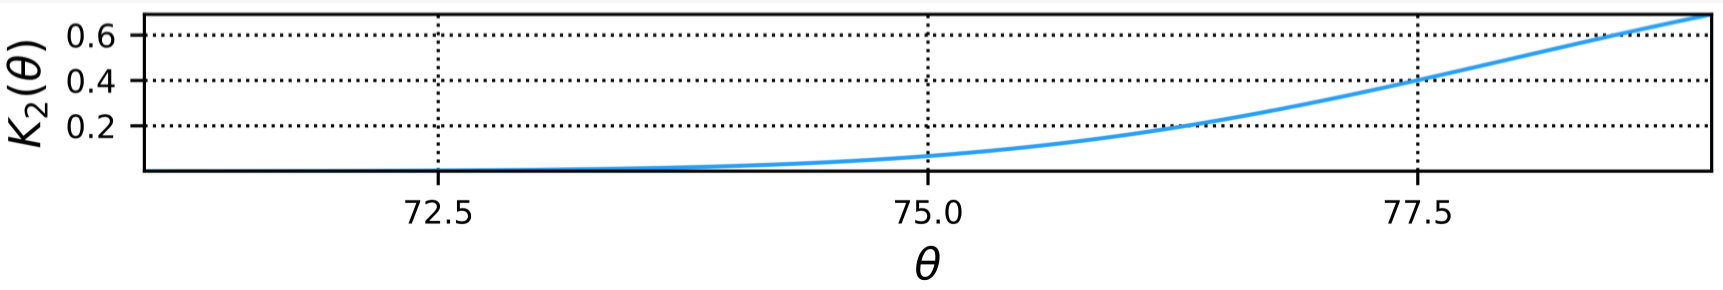
\includegraphics[width=11cm]{A2022.IDSEPC.SperimentazioneDeduzione/k2.png}
\end{center}

$$K_2(75) = 0.067; but K_2(77) = 0.309$$
If true $\theta = 77$ we accept $H_1: \theta = 75$ only with probability 0.309.

\vspace*{1cm}
\begin{center}
\textcolor{green}{\textit{Remember, this is just a trailer, you are not required to fully learn it right now $\ldots{}$}}
\end{center}

\end{frame}

%----------------------------------------------------------------------------------------
%----------------------------------------------------------------------------------------



\begin{frame}
{\centerline{Back to the example (6/9)}}
Finally, we try to generalize with Test 3:
$$C = \{ (x_1,\ldots, x_n): (x_1 + x_2 + \ldots + x_n > n*c) \}$$
where $c$ is some constant, $n$ sample size, again $\bar{X} \sim N(\theta, 100/n)$.

\vspace*{1cm}
\begin{center}
\textcolor{green}{\textit{Remember, this is just a trailer, you are not required to fully learn it right now $\ldots{}$}}
\end{center}

\end{frame}
%----------------------------------------------------------------------------------------

%------------------------------------------------


\begin{frame}
{\centerline{Back to the example (7/9)}}


But now we want the power function of the Test 3 to meet conditions: 
$$K_{3}(\theta) = \mathbb{P}(\bar{X}>c) = 1 - N\left(\frac{c-\theta}{10/\sqrt[]{n}}\right)$$
$$K_{3}(75) = 0.159; K_{3}(77) = 0.841; $$

\vspace*{1cm}
\begin{center}
\textcolor{green}{\textit{Remember, this is just a trailer, you are not required to fully learn it right now $\ldots{}$}}
\end{center}


\end{frame}
%----------------------------------------------------------------------------------------



%------------------------------------------------

\begin{frame}
{\centerline{Back to the example (8/9)}}

$$N\left(\frac{c-75}{10/\sqrt[]{n}}\right) = 0.159; N\left(\frac{c-77}{10/\sqrt[]{n}}\right) = 0.841; $$
Solution: $n=100; c=76.$ 

Note, $K_3(73) = 0.001; and K_3(79) = 0.999$.

\begin{center}  
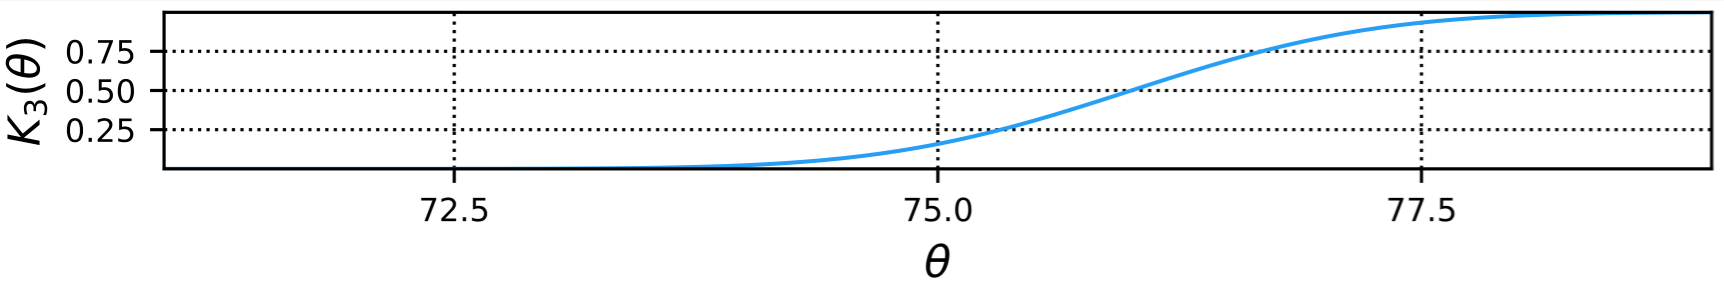
\includegraphics[width=11cm]{A2022.IDSEPC.SperimentazioneDeduzione/k3.png}
\end{center}

\vspace*{0.5cm}
\begin{center}
\textcolor{green}{\textit{Remember, this is just a trailer, you are not required to fully learn it right now $\ldots{}$}}
\end{center}

\end{frame}
%----------------------------------------------------------------------------------------



%------------------------------------------------

\begin{frame}
{\centerline{Back to the example (9/9)}}

Comparison of tests ($K_1, K_2,$ and $K_3$):
  
\begin{center}  
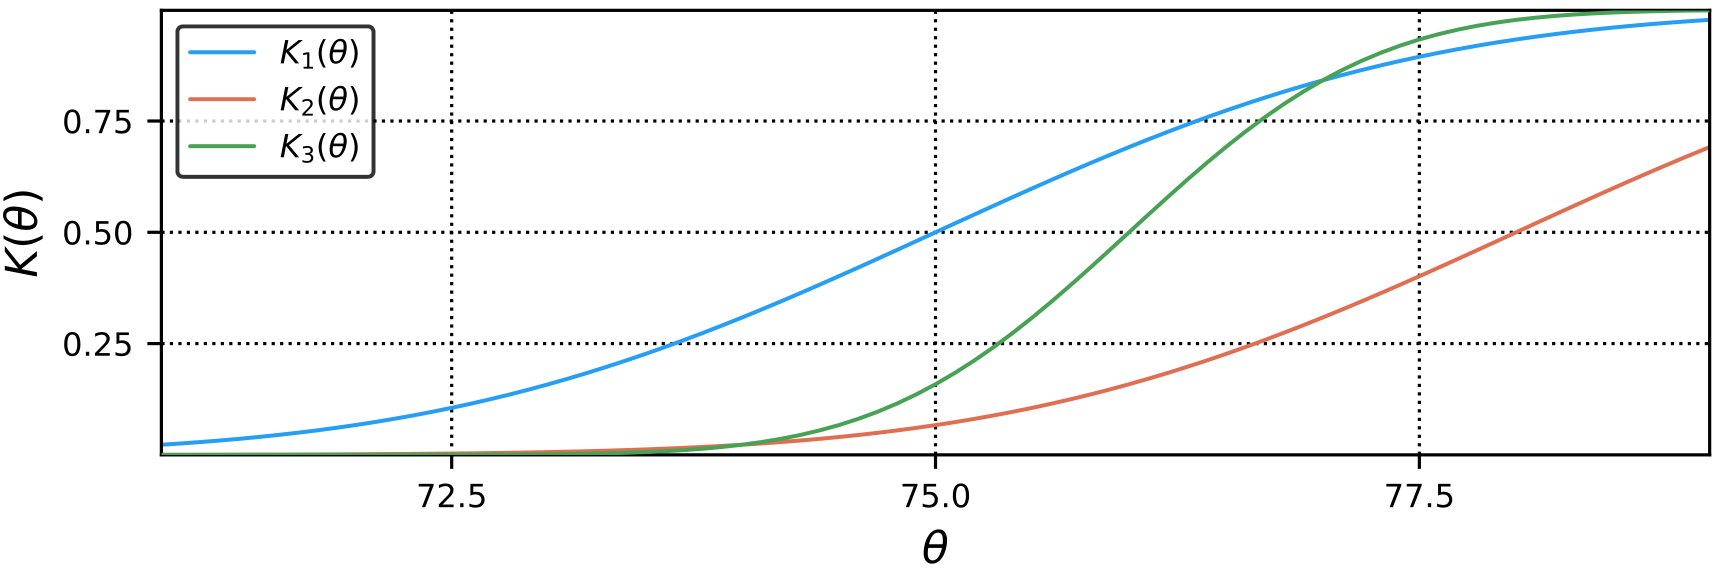
\includegraphics[width=11cm]{A2022.IDSEPC.SperimentazioneDeduzione/kk.png}

\end{center}

\vspace*{0.5cm}
\begin{center}
\textcolor{green}{\textit{Remember, this is just a trailer, you are not required to fully learn it right now $\ldots{}$}}
\end{center}

\end{frame}


%----------------------------------------------------------------------------------------
%------------------------------------------------

\begin{frame}
{\centerline{Hypothesis testing. Type I and II errors}}

%table
\begin{center}
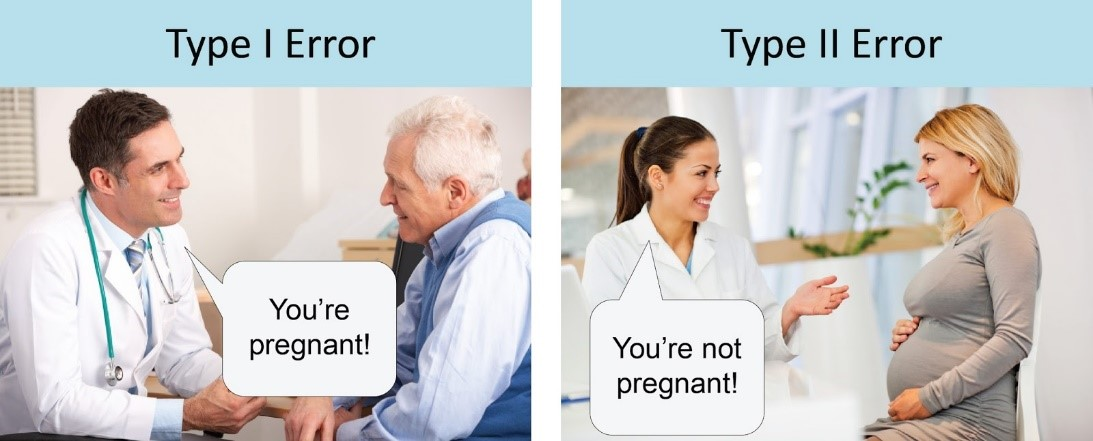
\includegraphics[height=4.5cm]{A2022.IDSEPC.SperimentazioneDeduzione/t1-t2-examples.jpg}
\end{center}

\vspace*{0.5cm}
\begin{center}
\tiny
Taken with modifications from: \url{https://www.statisticssolutions.com/wp-content/uploads/2017/12/rachnovblog.jpg}
\end{center}

\end{frame}

%----------------------------------------------------------------------------------------
%------------------------------------------------

\begin{frame}
{\small \centerline{Hypothesis testing. Hints for the terminology}}

The following concepts are all equivalent:
\begin{itemize}
\item ``significance level" 
\item ``size of the critical region"
\item ``power of the test when $H_0$  is true,"
\item ``the probability of committing an error of type I"
\end{itemize}

\end{frame}
%----------------------------------------------------------------------------------------
%------------------------------------------------



\begin{frame}
{\centerline{Domande?}}
\vspace{1cm}
\begin{center}
    \LARGE{Fine della lezione sei.}
\end{center}

\end{frame}

\end{document}


